\documentclass[aspectratio=169]{iticslides}
\AtBeginDocument{\selectlanguage{english}}

% --- Presentation Meta Data ---
\title{Federated Learning for Pneumonia Classification using GAN-Augmented Chest X-Rays}
\author{Pau Camos \& Daniel Alamillo}
\institute{Universitat Politècnica de Catalunya}
\date{Mini Project Proposal Defense}

\hypersetup{
  colorlinks=true,
  urlcolor=blue,
  linkcolor=black
}

\usepackage{caption}
\captionsetup{justification=centering}

\begin{document}

% --- Title Slide ---
\begin{frame}
  \titlepage
\end{frame}

\begin{frame}{Agenda}
  \tableofcontents
\end{frame}

\section{Context}

% --- Slide 1: Context & AI Challenges ---
\begin{frame}{Context: Challenges in Healthcare AI}
  This project illustrates the core challenges AI engineers face in
  healthcare environments:
  \begin{itemize}
  \item \textbf{Private Data:} Sensitive patient records cannot be centralized.
  \item \textbf{Distributed Data:} Information is spread across
    multiple distinct hospitals or organizations.
  \item \textbf{Unbalanced Datasets:} Scarcity of specific
    diagnostic classes (e.g. a rare diesease datapoint).
  \end{itemize}
  
  \textbf{Core Objective:} Modern CNNs easily achieve high accuracy
  for this specific classification. The true goal is
  demonstrating a robust, end-to-end AI pipeline that overcomes
  these systemic barriers.
\end{frame}

\begin{frame}{Context: Use Case (unbalanced Chest X-Ray classification)}
  \begin{itemize}
  \item \textbf{Task:} Binary classification of patient
    scans (Pneumonia vs. Normal).
    \vspace{0.3cm}
  \item Significant class imbalance due to a scarcity of the minority
    'NORMAL' class.
    
    \vspace{0.3cm}
    
  \item \textbf{Dataset Source:} \href{https://www.kaggle.com/datasets/paultimothymooney/chest-xray-pneumonia}{Chest X-Ray Images (Pneumonia) dataset}.
  \end{itemize}
\end{frame}

\section{System Architecture}

\begin{frame}{System Architecture: Solving the Challenges}
  \begin{itemize}
  \item \textbf{Generative Adversarial Network (GAN):}
    \begin{itemize}
    \item \textit{Solves Unbalanced Data:} A DCGAN architecture
      generates realistic synthetic images to augment the minority
      'NORMAL' class.
    \end{itemize}
    \vspace{0.3cm}
  \item \textbf{CNN Classifier:}
    \begin{itemize}
    \item \textit{Solves the Use Case:} Performs the binary
      diagnostic classification (Pneumonia vs. Normal).
    \end{itemize}

    \vspace{0.3cm}

  \item \textbf{Federated Learning (FL):}
    \begin{itemize}
    \item \textit{Solves Distributed Data:} Enables model training
      across simulated hospital clients without pooling data.
      
    \item \textit{Solves Privacy:} Only model weights are shared
      centrally via FedAvg, keeping raw data local.
      
    \end{itemize}
  \end{itemize}
\end{frame}

\begin{frame}{Generative Adversarial Network (GAN) (1)}
  \begin{columns}
    \begin{column}{0.55\textwidth}
      \begin{itemize}
        \item \textbf{Data Strategy}: Augments the minority class
          until it mathematically equilibrates with the 'PNEUMONIA'
          class count.
      
      \vspace{0.6cm}
      
      \item \textbf{Implementation Reference}: The core architecture
        is based on the official TensorFlow Deep Convolutional GAN
        (DCGAN) tutorial.
        \begin{itemize}
        \item \url{https://www.tensorflow.org/tutorials/generative/dcgan}
        \end{itemize}
      \end{itemize}
    \end{column}
    
    \begin{column}{0.45\textwidth}
      \begin{figure}
        \centering
        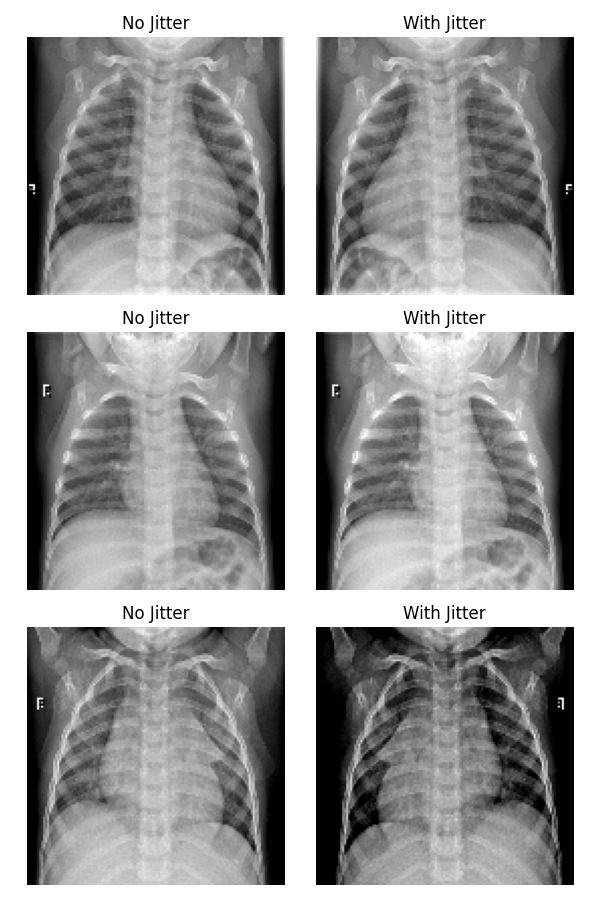
\includegraphics[width=0.55\textwidth]{media/compare_jitter.png}
        \caption{Preprocessing via jitter (horizontal flip, random brightness)}
      \end{figure}
    \end{column}
  \end{columns}
\end{frame}

% \begin{frame}{Generative Adversarial Network (GAN) (1)}

%   \begin{figure}
%     \centering
%     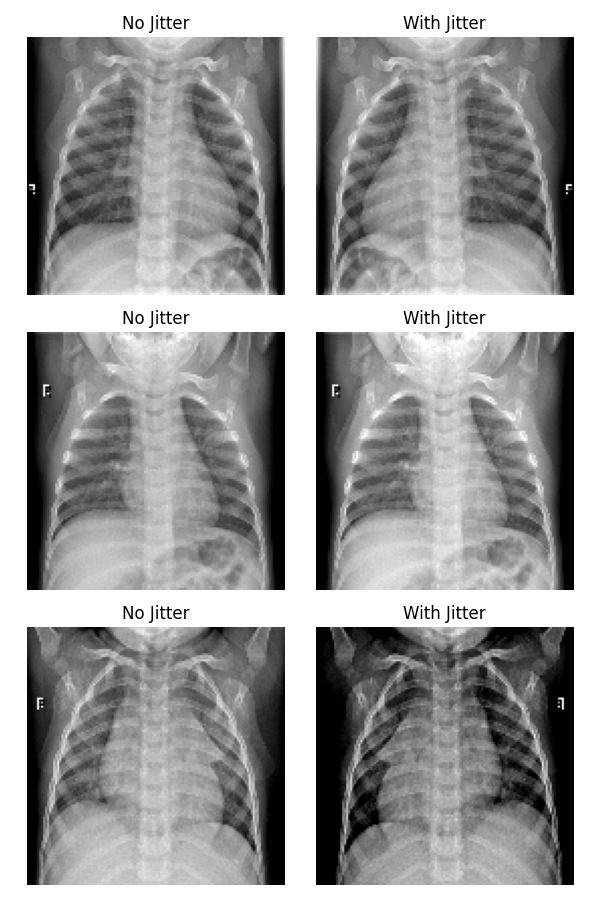
\includegraphics[width=0.3\textwidth]{media/compare_jitter.png}
%     \caption{Dataset preprocessing using jitter (horizontal flipping,
%       random brightness factor\dots)}
%   \end{figure}
% \end{frame}

\begin{frame}{Generative Adversarial Network (GAN) (2)}
  \begin{itemize}
  \item \textbf{Training Cycle}: 7,000 \texttt{epochs} sampling a
    100-dimensional noise vector.
    
  \item \textbf{Evaluation}: Fréchet Inception Distance (FID) computed
    via \texttt{InceptionV3} feature extraction. (Obtained score =
    $25$ (very accurate))
    
  \end{itemize}
  \begin{columns}
    \begin{column}{0.5\textwidth}
      \begin{figure}
        \centering
        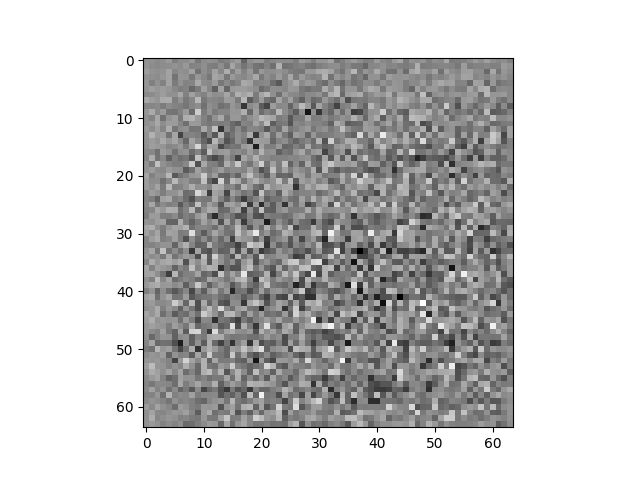
\includegraphics[width=0.5\textwidth]{media/generated_image_no_training.png}
        \caption{GAN generated image (without training)}
      \end{figure}
    \end{column}

    \begin{column}{0.5\textwidth}
      \begin{figure}
        \centering
        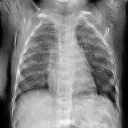
\includegraphics[width=0.5\textwidth]{media/restore_model_image_example.png}
        \caption{GAN generated image (after 7000 \texttt{epochs})}
      \end{figure}      
    \end{column}
  \end{columns}
\end{frame}

\begin{frame}{CNN Classifier}
  \begin{itemize}
  \item \textbf{Feature Extraction}: 4 sequential Convolutional blocks.
    \begin{itemize}
    \item \texttt{Conv2D} $\rightarrow$ \texttt{BatchNorm} $\rightarrow$ \texttt{LeakyReLU} $\rightarrow$ \texttt{MaxPool2D}.
    \item Filter depths: 32, 64, 128, 256.
    \end{itemize}
    
    \vspace{0.4cm}
    
  \item \textbf{Classification Head}: 
    \begin{itemize}
    \item \texttt{GlobalAvgPool2D} $\rightarrow$ \texttt{Dense(128)} (Dropout 0.5) $\rightarrow$ \texttt{Dense(1)}.
    \end{itemize}

    \vspace{0.4cm}

  \item \textbf{Training Setup}:
    \begin{itemize}
    \item \textbf{Optimizer}: Adam ($lr = 3 \times 10^{-5}$) with \texttt{ReduceLROnPlateau}.
    \item \textbf{Loss Function}: Binary Crossentropy.
    \item \textbf{Metrics}: Accuracy, AUC, Precision, Recall, F1-Score.
    \end{itemize}
  \end{itemize}
\end{frame}

\begin{frame}{Federated Learning (FL)}
  Executed via simulation using the following setup: 
  \begin{itemize}
  \item \textbf{Clients:} 4 independent nodes.
  \item \textbf{Data Split:} Randomly distributed (25\% of the dataset per client).
  \item \textbf{Training}
    \begin{itemize}
    \item \textbf{Local Execution:} 1 epoch per client per round.
      
    \item \textbf{Global Execution:} 50 total communication rounds
      (equivalent to the centralized baseline).
      
    \item \textbf{Synchronization:} Synchronous updates (nodes wait
      for all others to finish before starting the next round). 
    \end{itemize}

  \item \textbf{Model Aggregation Strategy:} FedAvg.
  \end{itemize}
\end{frame}

\section{Results}

\begin{frame}{Results: Centralized vs. Federated Training (1)}
  \begin{columns}
    \begin{column}{0.5\textwidth}
      \centering
      \textbf{Centralized Training AUC}
      \begin{figure}
        \centering
        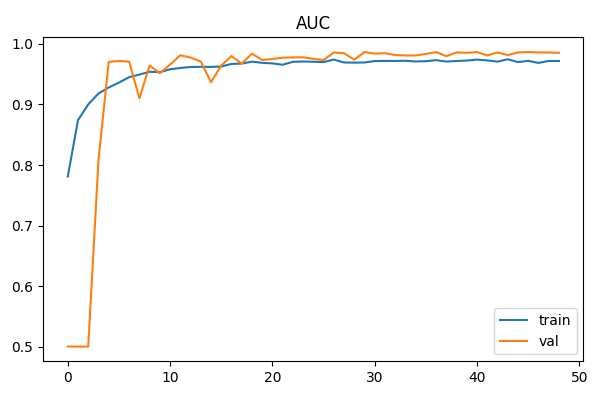
\includegraphics[width=\textwidth]{media/auc_centralized.png}
        \caption{Train Baseline Performance (AUC). \\ X-axis corresponds
          to \texttt{epochs}.}
      \end{figure}
    \end{column}
    
    \begin{column}{0.5\textwidth}
      \centering
      \textbf{Federated Training AUC}
      \begin{figure}
        \centering
        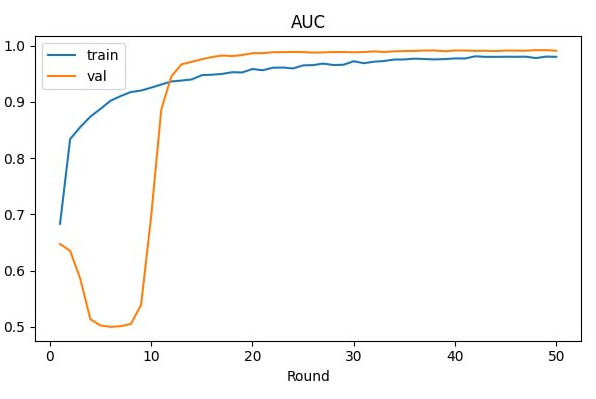
\includegraphics[width=\textwidth]{media/auc_federated.jpg}
        \caption{Train FL Performance (AUC). \\ X-axis corresponds to
          FL \texttt{rounds}.}
      \end{figure}

    \end{column}
  \end{columns}
\end{frame}

\begin{frame}{Results: Centralized vs. Federated Training (2)}
  \begin{columns}
    \begin{column}{0.5\textwidth}
      \centering
      \textbf{Centralized Training Loss}
      \begin{figure}
        \centering
        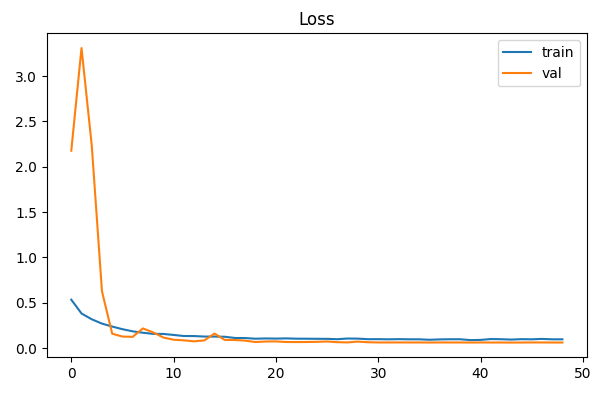
\includegraphics[width=\textwidth]{media/loss_centralized.png}
        \caption{Train Baseline Performance (AUC). \\ X-axis corresponds
          to \texttt{epochs}.}
      \end{figure}
    \end{column}
    
    \begin{column}{0.5\textwidth}
      \centering
      \textbf{Federated Training Loss}
      \begin{figure}
        \centering
        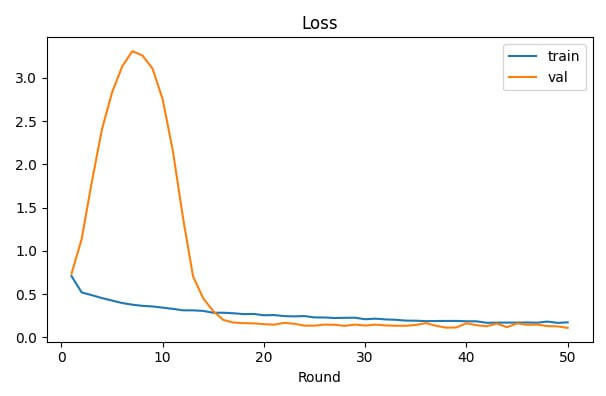
\includegraphics[width=\textwidth]{media/loss_federated.jpg}
        \caption{Train FL Performance (Loss). \\ X-axis corresponds to
          FL \texttt{rounds}.}
      \end{figure}
    \end{column}
  \end{columns}
\end{frame}

\begin{frame}{Results: Centralized vs. Federated Training (3)}
  \begin{columns}
    \begin{column}{0.5\textwidth}
      \begin{itemize}
      \item \textbf{Centralized:}

        \begin{itemize}
        \item Centralized Test Accuracy: 83.7\%
        \item Centralized Test AUC: 77\%
        \item Centralized Test Recall: 93\%
        \end{itemize}
      \end{itemize}
    \end{column}

    \begin{column}{0.5\textwidth}
      \begin{itemize}
      \item \textbf{Federated:}
        \begin{itemize}
        \item Federated Test Accuracy: 81\%
        \item Federated Test AUC: 90\%
        \item Federated Test Recall: 92\%
        \end{itemize}
      \end{itemize}
    \end{column}
  \end{columns}
\end{frame}

\section{Conclusions}

\begin{frame}{Conclusions}
  \begin{itemize}
  \item \textbf{Synthetic data generated successfully}: To
    equilibrate the dataset ($FID_{score} = 25$)

    \vspace{0.3cm}
    
  \item \textbf{Built CNN with good classification metrics}: That
    solves the main use case.

    \vspace{0.3cm}
    
  \item \textbf{Distributed training pipeline set up}: Giving the same
    or better results.
    
    \vspace{0.3cm}
  \item \textbf{Healthcare Extensibility:} This framework can be
    directly adapted to other sensitive medical domains.
    
  \end{itemize}
\end{frame}


\section{Q\&A}

\begin{frame}{Questions \& Answers}
  \begin{center}
    \vspace{1cm}
    {\LARGE \textbf{Thank you for your attention!}}
    
    \vspace{1.5cm}
    \textit{Pau Camos \& Daniel Alamillo}
  \end{center}
\end{frame}

\end{document}